\documentclass[]{article}
\usepackage{graphicx}
\usepackage{geometry}
\geometry{
	a4paper,
	total={170 mm, 257mm},
	left=30mm,
	right=35mm,
	top=20mm,
}
%opening
\title{Phy117 Lab 3}
\author{Shijia (Scarlett) Yu \\Partner: Nishi\\Prof. Musumeci; TA: Albert Brown}
\date{January 28, 2017}

\begin{document}
	\maketitle
	\paragraph { (a)} %\mbox{}\\
	We used the "Fast Fourier Transform (FFT)" feature in the math menu, and obtained the FFT for 1kHz sine wave (Fig.1).
	\begin{center}
		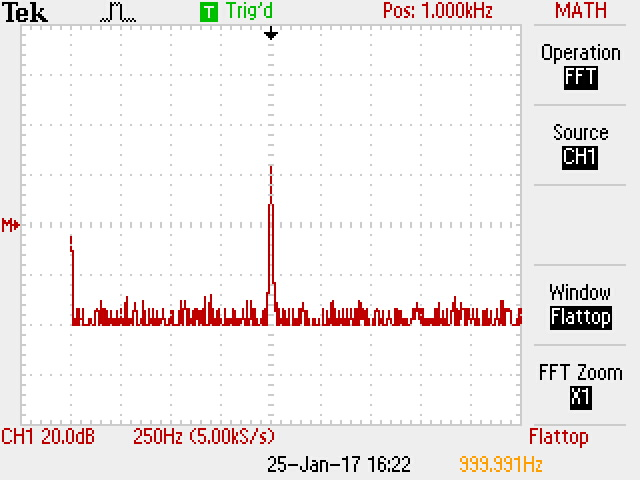
\includegraphics[scale=0.8]{a_sineFFT}\\
		Figure 1: Fast Fourier Transform for sine wave.
	\end{center}
	We also obtained the FFT for 1kHz square wave (Fig.2).
		\begin{center}
			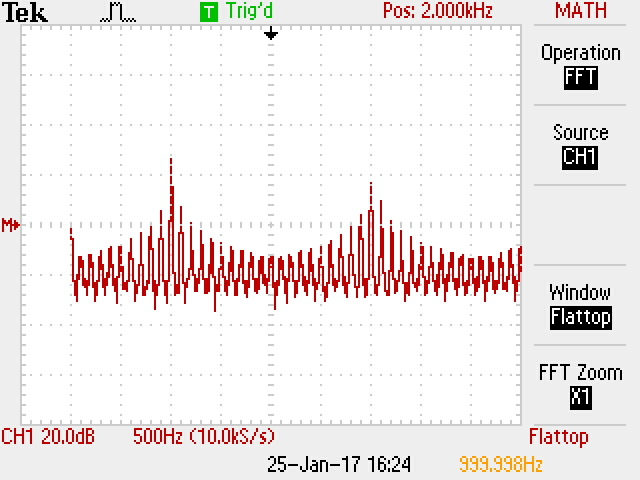
\includegraphics[scale=0.8]{a_squareFFT}\\
			Figure 2: Fast Fourier Transform for square wave.
		\end{center}
	The fast Fourier Transform represents the fourier transform of a function of time in frequency space. So in the FFT of sine wave, we see that the power falls on one frequency and which is the frequency that contributes the most to the approximation of the sine wave. Similarly since the Fourier coefficients of square wave are odd, and the higher the coefficient the less they contribute to the approximation, as we saw on the scope, only certain frequencies peak out and the consecutive peak has lower amplitude than the previous peak.\\ \\ \\ \\ \\ \\
	\paragraph{ (b)} 	
We built the LC circuit below (Fig.3) and drove it with 1kHz sine wave at 1V. We used CH1 of the scope for the output signal and CH2 for fucntion generator's input signal. 
\begin{center}
	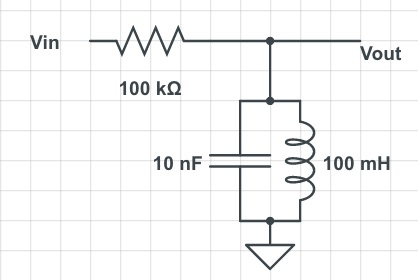
\includegraphics[scale=0.5]{b_circuit}\\
	Figure 3: LC circuit passband
\end{center}
The calculated resonant frequency for this circuit is $f_{r}=\frac{1}{2\pi \sqrt{LC}}=\frac{1}{2\pi \sqrt{0.01H \times 10^{-12}F}}=16 kHz$. On the fucntion generator, we varied the driving frequency around 16kHz by turnung the knob unitl we saw resonance on the scope (Fig.4). In this way, the measurened resonant frequency is 16.3kHz. So, due to damping, the measured peak of the passband is off from our calculated value by $16.3 kHz-16 kHz=0.3 kHz$, which is $\frac{0.3}{16.3}=1.8\%$ relative error.
\begin{center}
	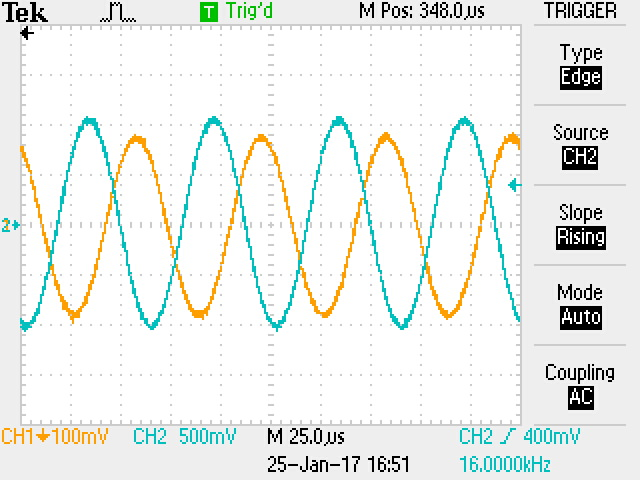
\includegraphics[scale=0.8]{b_resonance}\\
	Figure 4: Resonance of LC circuit at 16.3 kHz.
\end{center}
Then we drove the circuit below $f_{r}$ at 8 kHz (Fig.5) and above $f_{r}$ at 26kHz (Fig.6).
\begin{center}
	\includegraphics[scale=0.8]{b_8Hz}\\
	Figure 5: Below the resonant frequency of LC circuit at 8kHz.
\end{center}

\begin{center}
	\includegraphics[scale=0.8]{b_26Hz}\\
	Figure 5: Above the resonant frequency of LC circuit at 26 kHz.
\end{center}

	\paragraph{ (c)} 	
	Continuing from part (b), now we set the fucntion generator to linear sweep mode, sweeping from 5 kHz to 25 kHz, with $\Delta t=1s$. We also connected SYNC to CH3 of the scpoe and set the trigger on SYNC. Looking at the peak detect of the output signal, we saw that at one particular frequency, which is the resonant frequency, the amplitude peaks out. 
	\begin{center}
		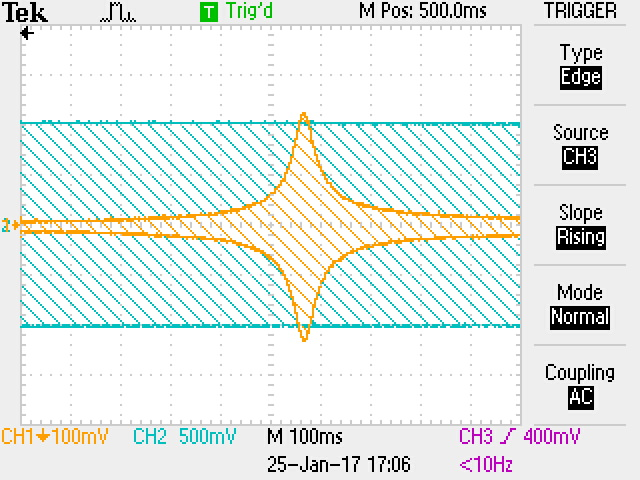
\includegraphics[scale=0.8]{c_qfactor}\\
		Figure 6: Voltage vs. Time of  the passband by sweeping from 5 kHz-25 kHz
	\end{center}
	Now we can calculate the Q factor $Q=\frac{f_{res}}{\Delta f}$ from Fig.6. First we need to find the measured $f_{res}$ here. The freqency sweep range is $25 kHz-5 kHz=20 kHz$. The time at the peak resonant frequency in Fig.6 is 0.568s.  So the measured resonant frequency is $f_{res}= f_{starting}+\delta f=5 kHz+ (20kHz\times 0.568s)=5 kHz+11.3 kHz=16.3kHz$, which agrees with our measured values in part (b) as it should.  \\ \\ Then we need to find $\Delta f$, the full-width at half-maximum. Using the cursors, we found $V_{max}=224V$, so $V_{3dB}=224V\times 0.707=158V$. We used the cursors and found the time $t_{1}=0.548s$ and $t_{2}=0.584s$ at the two 3dB voltages, respectively. So, just as how we calculated the resonant frequency, now we have $f_{1}=20 kHz\times 0.548s=15.96 kHz$, and $f_{2}=20 kHz\times 0.584s=16.68kHz$. Therefore, $\Delta f=16.68kHz-15.96 kHz=0.72 kHz$. \\The Q-factor is then $Q=\frac{16.3 kHz}{0.72 kHz}=22.7$. 
	\paragraph{ (d)} 	
	Continuing with the same LC circuit, we then drove it with a square wave at 1kHz ( (a long period) and 1V. At the edge of the square wave, which is where we "whack" the circuit because there's a sharp change of voltage, we saw some resonance (Fig.7).
		\begin{center}
			\includegraphics[scale=0.8]{D_resonance}\\
			Figure 7: Resonance at the edge of square wave, where the circuit is "whacked".
		\end{center}
	The resonace occurs here because since there's a rapid change of voltage, which is like a AC signal, the LC circuit will respond to it and show resonance at the trasisition edge. Zooming in on the resonace (Fig.8), we can procceed to find the resonant frequency and Q-factor using energy lost per cycle.
	\begin{center}
		\includegraphics[scale=0.8]{D_qfactor}\\
		Figure 8: Zoomed in on resonance to find resonant frequency and Q-factor.
	\end{center}
	Using the cursors, we found the $\Delta t $ bewtween two peaks is $\Delta t= 77\mu s-15\mu s=62\mu s$. So by definition, the frequency can be calculated: $f=\frac{1}{\Delta t}=1/62\mu s=16.1 kHz$, which is what we expected.\\
	To find the Q-factor, we used the definition $Q=2\pi \frac{Energy \ stored}{Energy \ disspated \ per \ cycle}$. All the energy in the circuit is stored in capacitor plus inductor, but when at peak voltage, all the energy is on capacitor. Then voltage at the first peak in Fig.8 is 20.4mV.  So, the total energy is
	\[  E_{tot}=E_{C}=\frac{1}{2} CV_{peak}^{2}=\frac{1}{2} (0.01\times 10^{-6}F) (20.4\times 10^{-3}V)^{2}= 2\times 10^{-12}J \]
	The enegy lost can be calculated from the damping of the oscillation. The voltage at the second peak in Fig.8 is 17.2 mV. So, the energy lost in one cycle is:
	\[\Delta E=  \frac{1}{2} C(V_{1}^{2}-V_{2}^{2}) =\frac{1}{2}(0.01\times 10^{-6}F)[(20.4 \times 10^{-3}V)^{2}-(17.2 \times 10^{-3}V)^{2}]=6.016\times 10^{-13}J \]
	Thefore, the Q-factor is: $2\pi \times \frac{2\times 10^{-12}J}{6.016\times 10^{-13}J}=21$, which is close to 22.7 we got in part (c).\\
	\paragraph{ (e)}	
	We driove the LC circuit with square waves at resonant frequecy of 16.3 kHz. We saw that certain the sine wave signal peaked out (Fig.9). This is because only frequencies near the resonant frequency of the passband circuit will pass, therefore, only frequency of sine wave near 16 kHz will show up.
		\begin{center}
			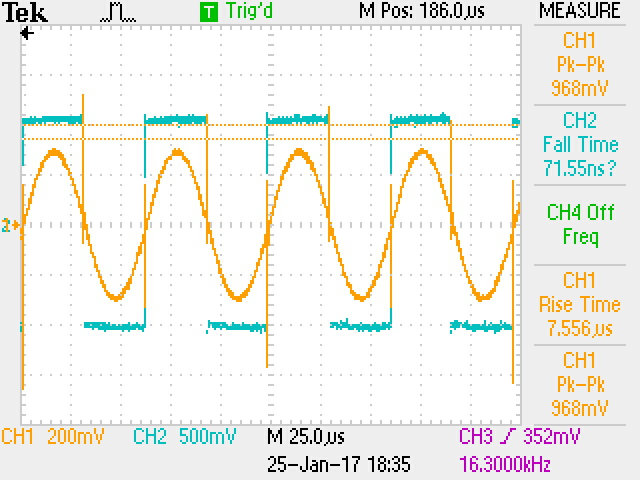
\includegraphics[scale=0.8]{e_squareResonance}\\
			Figure 9: Driving LC circuit at fundamental resonant frequency of 16 kHz.
		\end{center}
	Then we changed the frequency around until we saw another peak repsonse at 5.43 kHz (Fig.10), another resonance frequency. We set 16 kHz to be our fundamental harmonic, so 5.43 kHz, which is about 1/3 of the fundamental, is then the first harmonic.
		\begin{center}
			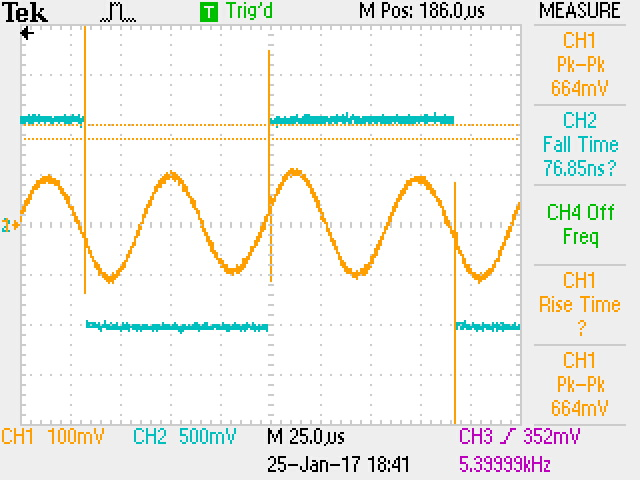
\includegraphics[scale=0.8]{e_54hz}\\
			Figure 10: Driving LC circuit at resonant frequency of 5.43 kHz (first harmonic).
		\end{center}
		Going down by around 1/5 of the 16 kHz fundamental, we found the second harmonic at 3.26 kHz resonant frequency (Fig.11).
			\begin{center}
				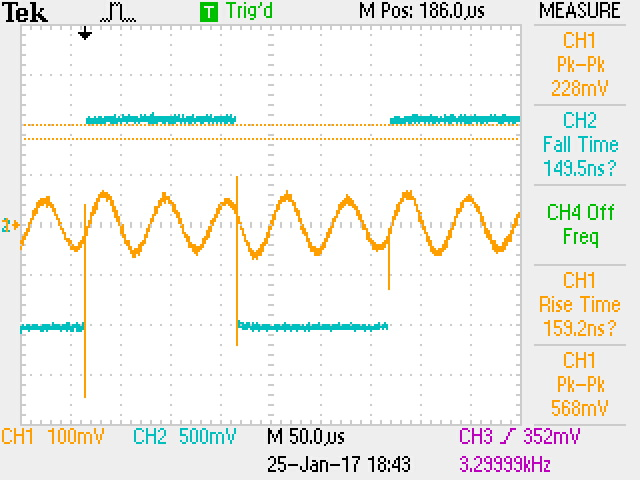
\includegraphics[scale=0.8]{e_33hz}\\
				Figure 11: Driving LC circuit at resonant frequency of 3.26 kHz (second harmonic).
			\end{center}
		Similarly, going down by around 1/7 and 1/9 of the fundamental we found the third harmonic at 2.33kHz (Fig.12), and the forth harmonic at 1.8 kHz (Fig.13). 
		\begin{center}
			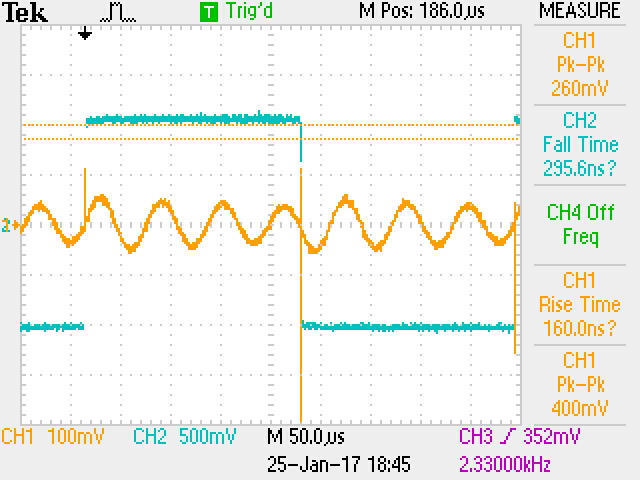
\includegraphics[scale=0.8]{e_233hz}\\
			Figure 12: Driving LC circuit at resonant frequency of 2.33 kHz (third harmoic).
		\end{center}
		\begin{center}
			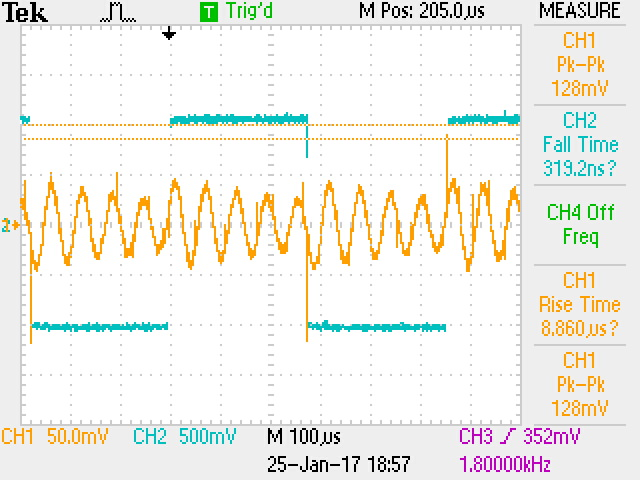
\includegraphics[scale=0.8]{e_18hz}\\
			Figure 13: Driving LC circuit at resonant frequency of 1.8 kHz (fourth harmoic).
		\end{center}

	\paragraph{ (f)} 	
	We built a half-wave recitifier below (Fig.14) using a 1N914 diode and 2.2k resistor in series. 
		\begin{center}
			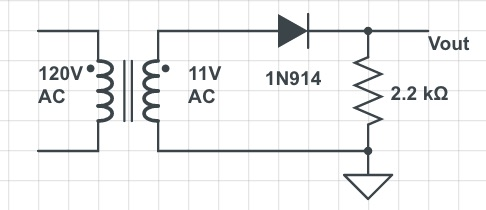
\includegraphics[scale=0.4]{f_circuit}\\
			Figure 14: Half-wave rectifier circuit
		\end{center}
	How this circuit works: The 120 AC voltage comes from the power supply on the wall, and transformer reduces it to 11 AC. As the current flows, only the one direction of the AC current is allowed to pass through the diode and diode also causes a 0.6V voltage drop. This means that current must start positively at the left of the diode in Fig.14, flows through the diode to the resistor. Therefore, we should expect to see only positive half cycle of the AC current arrives at $V_{out}$. \\On the scope, we indeed saw that the CH2 output is half of the original input signal and it's positive (Fig.15).
\begin{center}
	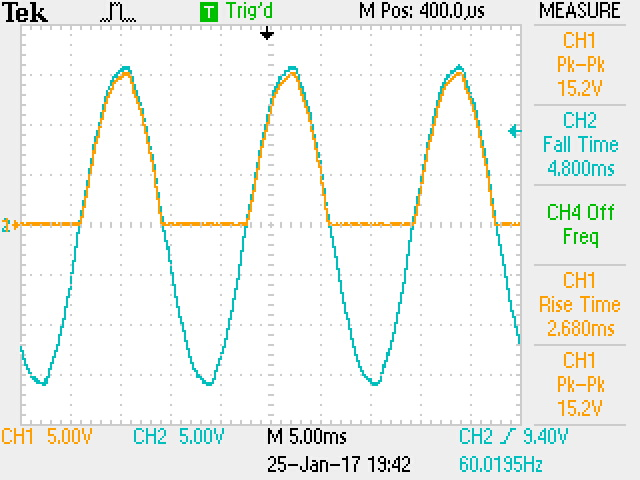
\includegraphics[scale=0.65]{f_halfrectifier}\\
	Figure 15: Half-wave rectifier output signal
\end{center}
To flip the polarity of the circuit, meaning if we only want the output signal to be negative, we can flip the direction of the diode in Fig.14 circuit to make it point to the left instead of right. In this way, the negative half-cycle of the AC current will pass through the diode.
	\paragraph{ (g)} 	
	To build a full-wave rectifier, we connected 4 diodes and the load as shown in Fig.16.
	\begin{center}
		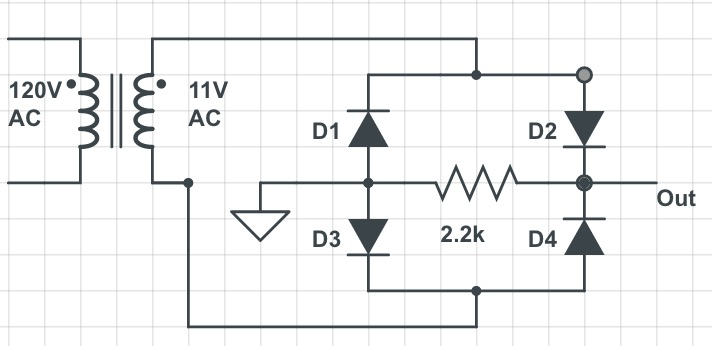
\includegraphics[scale=0.35]{g_circuit}\\
		Figure 16: Full-wave rectifier 
	\end{center}
	The CH1 of the scope is connected from $V_{out}$ to ground, so it's getting the output signal across the whole full-wave rectification circuit. CH3 is connected from the top node bewtween D1 and D2 to ground, so it's only across D2 and D3. Lastly, CH4 is connected from the bottom node between D3 and D4, so it's reading output across D1 and D4. In this way, we saw that in CH3 and CH4 both rectified half wave and resulted in positive half-cycle, but the resulting waves were shifted by 90 degrees with each other.
	Using the math mode on the scope, we subtracted CH3 from CH4, obtaining the original full wave (Fig.17).
	\begin{center}
		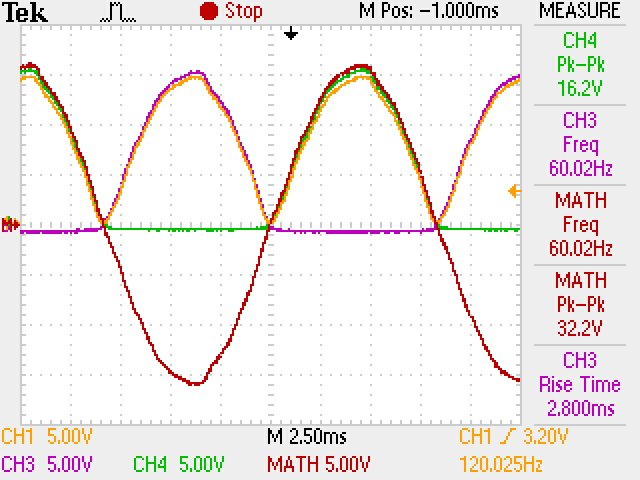
\includegraphics[scale=0.8]{g_subtract}\\
		Figure 17: Original full wave obtained by subtracting CH3 from CH4.
	\end{center}
Finally, note that to flip the polarity of this circuit, we will just need to switch $V_{out}$ with ground, or alternatively and more laboriously, flip the directions of all four diodes.
		
	\paragraph{ (h)} 	
	Now we replaced the diodes with LEDs as shown in Fig.18.
		\begin{center}
			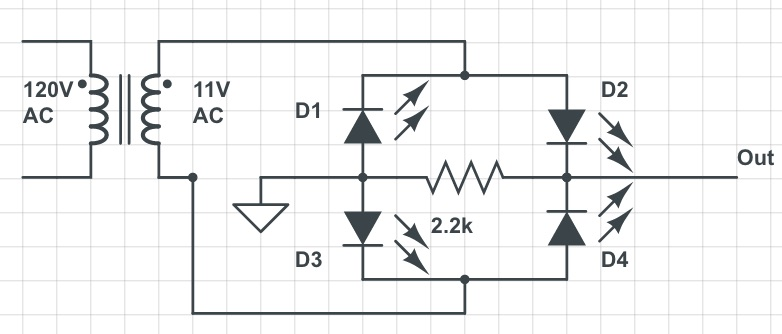
\includegraphics[scale=0.3]{h_circuit}\\
			Figure 18: Full-wave rectifier with LEDS.
		\end{center}
	We drove the circuit with a 0.5 Hz sine wave and 0.9V. We saw the that the two adjacent LEDs (D1 \& D4, D2 \& D3) light up alternatingly every 2 seconds, as the AC voltage flipped its sign. 
	\paragraph{ (i)} 	
	We connected a 15$\mu F$ electrolytic capacitor to the output of the full-wave rectifier circuit we built in part (g). What we expected the output signal to be: Since we have AC power, when the diode is forward biased (positive current flowing through the diode), the capcitor charges up, so the voltage signal here should be linearly increasing. When the AC voltage flips, the diode is reverse biased, no current flows through the diode and the capacitor discharges, so the voltage signal should be linearly decreasing. Therefore, overall we should see a sawtooth-like ripple signal. On the scope, we indeed saw such ripple (Fig.19)
		\begin{center}
			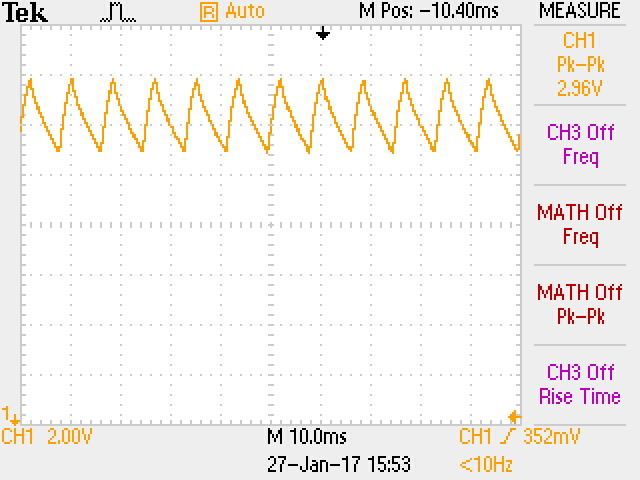
\includegraphics[scale=0.8]{i_ripple}\\
			Figure 19: Ripple in output signal of full-wave retification on capacitor
		\end{center}
	If we use a larger capacitor in the circuit, the ripple will be smaller, because larger capacitance the dischage and charge curve will be less steep.
	\paragraph{ (j)} 	
	We built the "diode-clamp"circuit as shown in Fig.20, which consists of a RC differentiator (high-pass filter) connected to a diode that rectifies the output signal of the differentiator. We drove the circuit with a 10kHz and 5V square wave.
	\begin{center}
		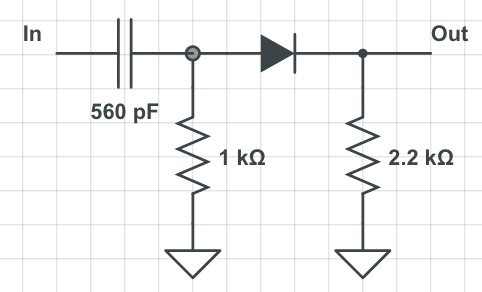
\includegraphics[scale=0.4]{j_circuit}\\
		Figure 20: Circuit that rectifies the output of differentiator.
	\end{center}
	We saw before that if we input a square wave to the differentiator, the differentiated signal would be a symmeteric triangular-like wave with positve and negative peaks, as the capacitor charges up and dischrges. So here with the diode to rectify, the final output signal should only be positive, meaning the nagative part of the differentiated wave will be clamped off. The signal we saw on the scope (Fig.21) matches our expectation. 
		\begin{center}
			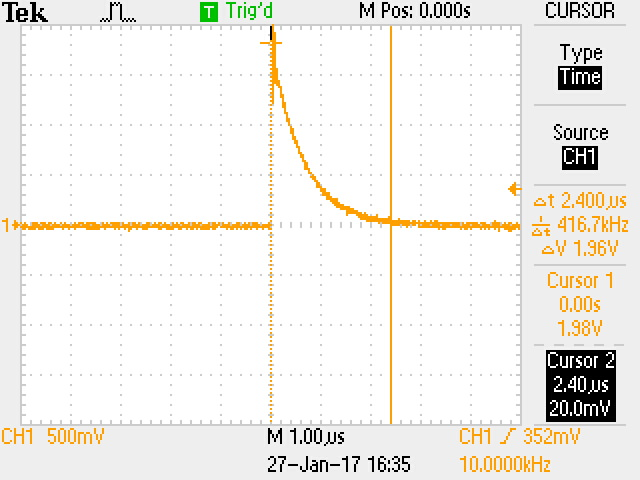
\includegraphics[scale=0.8]{j_rcdischarge}\\
			Figure 21: RC discharge curve of the rectified differentiator.
		\end{center}
The 2.2k resistor is there in the circuit because if we remove it, the resistance in the cirucit will increase a lot, so the RC time constant will also go up a lot. 
	\paragraph{ (k)} 	
	We built the circuit as shown in Fig.22, with a 1k resistor and a 1N914 diode in series. The +5V below the diode provides a baseline voltage, meaning that, since there is also a 0.6V drop across diode, the diode works only when the input voltage is greater than 5.6V. 
		\begin{center}
			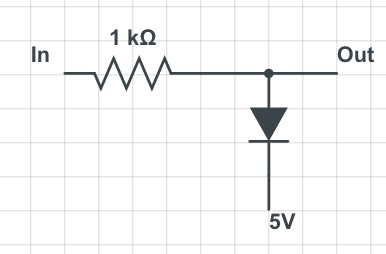
\includegraphics[scale=0.4]{k_circuit}\\
			Figure 22: "Diode-clamp" circuit.
		\end{center}
We first drove the circuit with a sine wave of 2V. Since 2V is below 5.6V, we expect the output to be the same as input signal since the diode should be off. On the scope, we saw the input and output signals overlap (Fig.23) with each other, so they indeed looked the same.
		\begin{center}
			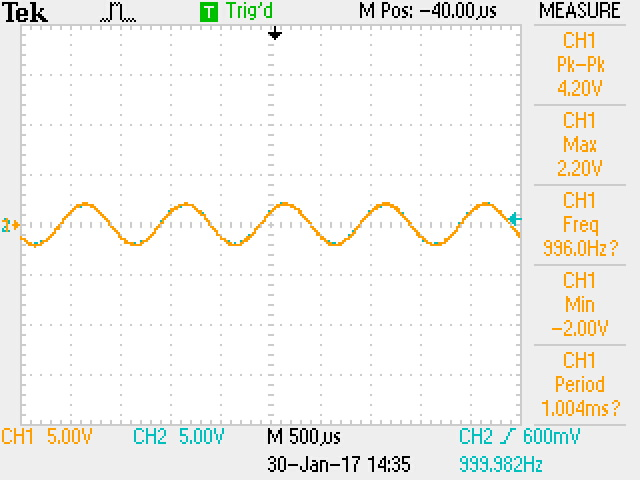
\includegraphics[scale=0.8]{k_below}\\
			Figure 23: Driving the diode clamp circuit with 2V.
		\end{center}
Now we drove the circuit with sine wave at 10V, which is above 5.6V. We saw on the scope (Fig.24) thatthe diode now worked as a clamp, keeping the voltage at the baseline +5V.
\begin{center}
	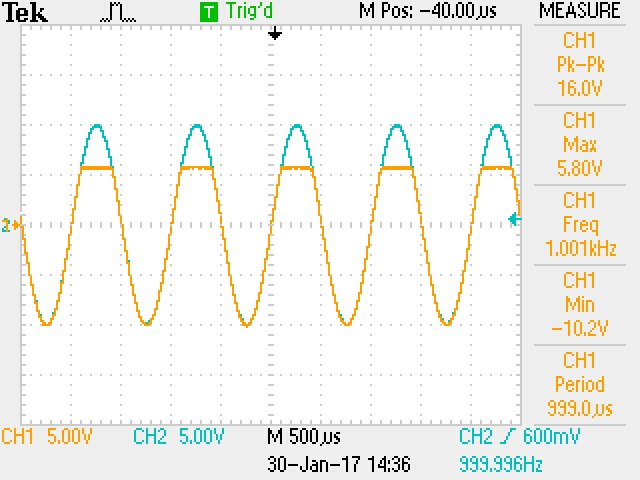
\includegraphics[scale=0.8]{k_above}\\
	Figure 24: Driving the diode clamp circuit with 10V.
\end{center}
	\paragraph{ (l)} 	
Now we built the "diode-limiter" circuit as shown in Fig.25. 
\begin{center}
	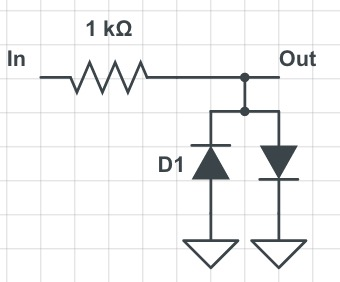
\includegraphics[scale=0.35]{l_circuit}\\
	Figure 25: "Diode-limiter" circuit 
\end{center}
In the circuit, the D1 diode is backward biased, clampping the nagative half cycle of the input signal at -0.6V. The other diode is forward biased, clamping off the positive cycle of the signal at +0.6V. 
\\We drove the circuit with 2V of sine waves, on the scope (Fig.26), the orignal wave is at $\pm 2V$, the output signal, however, is clamped at around $\pm$0.6V.
\begin{center}
	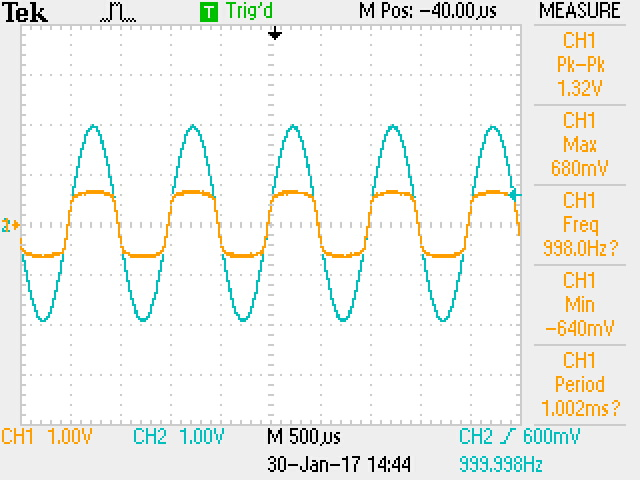
\includegraphics[scale=0.8]{l_sine}\\
	Figure 26: Sine wave inputted into "diode-limiter" 
\end{center}
	Similarly, we drove the circuit with 2V square waves (Fig.27), triangular waves (Fig.28), and saw-tooth waves (Fig.29). As expected, for all the functions the input signals oscillated between $\pm 2V$, whereas the output signals were between $\pm 0.6V$.
\begin{center}
	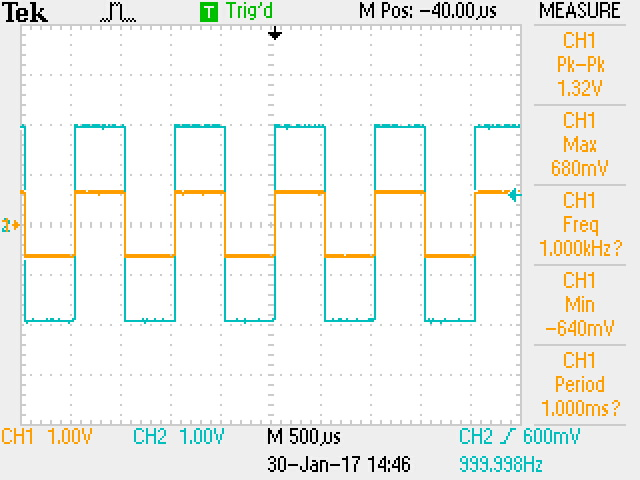
\includegraphics[scale=0.8]{l_square}\\
	Figure 27: Square wave inputted into "diode-limiter" 
\end{center}

\begin{center}
	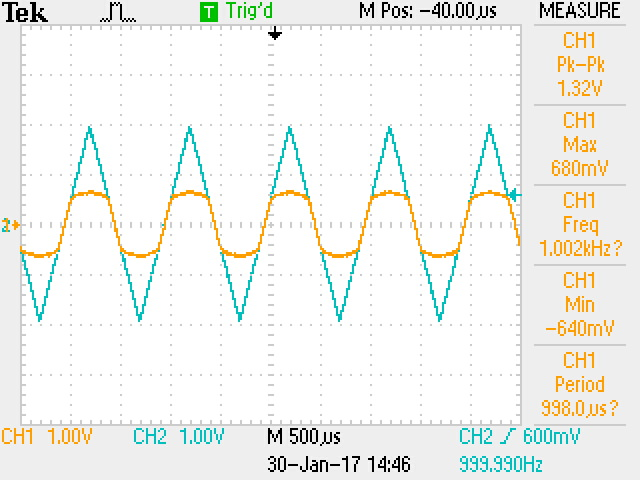
\includegraphics[scale=0.8]{l_triangle}\\
	Figure 28: Triangular wave inputted into "diode-limiter" 
\end{center}

\begin{center}
	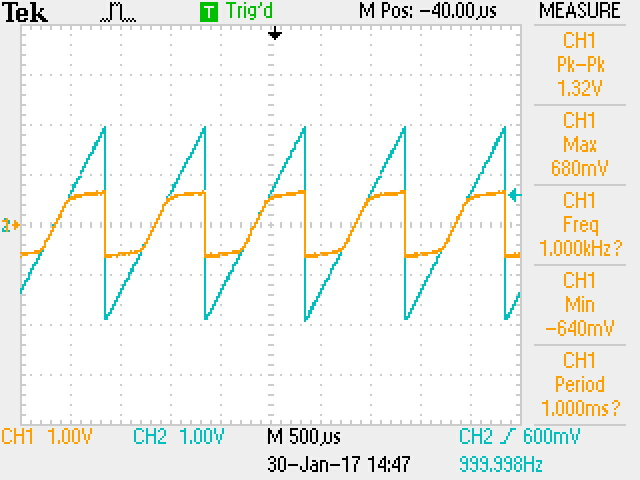
\includegraphics[scale=0.8]{l_sawtooth}\\
	Figure 29: Saw-tooth wave inputted into "diode-limiter" 
\end{center}
	\paragraph{ (m)}
We connected the scope probe to the oscilloscope, and connected an Ohm-meter across the scope probe. Wehn the scope probe is at $\times 1$ setting, the Ohm-meter read 1.00M$\Omega$. When we put the probe to $\times 10$ setting, the Ohm-meter read 9.98 M$\Omega$, which is about 10 times the resistance before as expected. 
	\paragraph{ (n)} 	 	
To test if a diode is Zener diode, we can backward biased the unknown diode (Fig.30). 
\begin{center}
	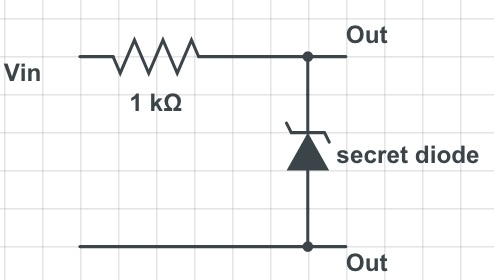
\includegraphics[scale=0.4]{n_circuit}\\
	Figure 30: Circuit setup to test Zener diode. 
\end{center}
If the diode is regular diode, no current will pass through and we should not be seeing any signal on the scope. But if it's a Zener diode, the signal will get through and the diode will clamp both the positive and negative cycles of the input signal. 
\\We were given a secret diode, we connected it backwards in the circuit, and saw on the scope (Fig. 31) that the output signal as recitified both on the top and bottom.  So the secret diode was a Zener diode. 
\begin{center}
	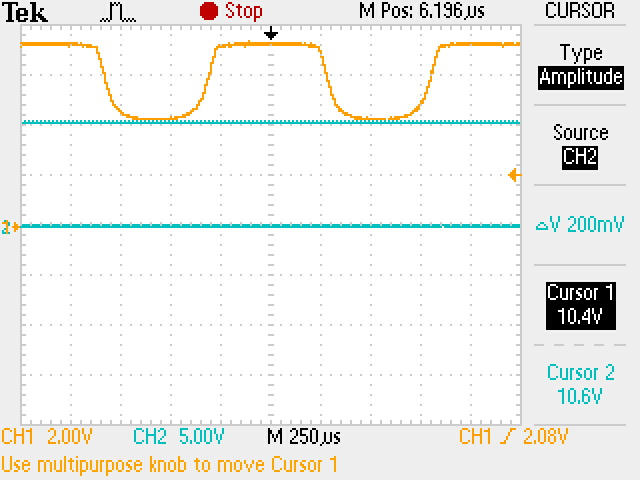
\includegraphics[scale=0.8]{n_zener}\\
	Figure 31: Output signal of the secret diode.
\end{center}
To determine the breakdown voltage of the Zener diode, we looked negative part at the rectified signal in Fig.31, because that's where the breakdown region of the Zener diode. So we wanted to know what that negative constant voltage is. Counting the division in Fig.31, the bottom line of the signal is at around 4V. Subtracting the 0.6V drop across the diode, the breakdown voltage is, therefore, 3.4V. 
\end{document}
